\documentclass{article}[12pt]
\usepackage{graphicx} % Required for inserting images
\usepackage{listings}
\usepackage{hyperref}
\usepackage{tabularx}
\usepackage{float}
\title{EARIN Lab 3 Report}
\author{Krzysztof Rudnicki, 307585 \\ Jakub Kliszko, 303866  }
\date{\today}

\begin{document}

\maketitle

\section{Exercise Variant 2 - "Rastrigin function"}
Our task was to write a program that optimizes Rastrigin function: \\
\[ f (x, y) =
20 + (x^2 - 10 \, cos(2πx)) + (y^2 - 10 \,  cos(2πy)) \]
Using Evolutionary Strategy ($\mu$, $\lambda$) (later refered as ES($\mu$, $\lambda$)) \\ 

\section{Implementation}
Program can be ran by installing python, moving to project directory and issuing command:
\begin{lstlisting}[language=bash]
python main.py
\end{lstlisting}
There are 7 parameters we can (but do not have to) change:
\begin{enumerate}
\item Number of parents (default equal to 5)
\item Size of population (default equal to 20)
\item Mutation Strength (default equal to 0.1)
\item Number of generations (default equal to 100)
\item Minimal Value (default equal to -5.12)
\item Maximal Value (default equal to 5.12)
\item Number of outputs (default equal to 10)
\end{enumerate}
Number of outputs are strictly for displaying results and does not influence the result itself \\ 
To set parameters values user can add those flags to program run:
\begin{lstlisting}[language=bash]
    -nop --number_of_parents [number]
    -sop --size_of_population [number]
    -ms --mutation_strength [number]
    -nog --number_of_generations [number]
    -min --min_value [number]
    -max --max_value [number]
    -noo --number_of_outputs [number]
\end{lstlisting}
Order of those parameters does not matter, user can provide none, one, or any number of arguments \\ 
Exemplary use (settings all values to default values):
\begin{lstlisting}[language=bash]
    python main.py -nop 5 -sop 20 -s 0.1
    -i 100 -min -5.12 -max 5.12 -noo 10
\end{lstlisting}
To print help info about program user can issue help flag:
\begin{lstlisting}[language=bash]
    python main.py -h
\end{lstlisting}
Results will be displayed on 2D scatter plot. There will be as many outputs as user wanted with incrementation of generation so that the final plot will be on final generation \\ 
\begin{figure}[H]
    \caption{Exemplary plot halfway through generation with parameters \\ nop 250 sop 1000 ms 0.1 nog 500 min max (-5.12, 5.12) }
    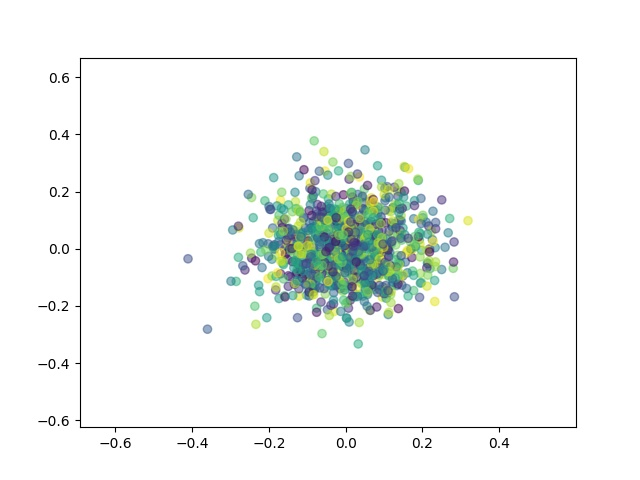
\includegraphics[width=8cm]{example_halfway.jpg}
    \centering
    \end{figure}
At the end summary of results on plot will display with red gradient showing results from the earliest (white) to latest (bright red) \\  
Results will be displayed and saved in the same folder as code directory for further inspection, with file name containing information about input parameters 
\section{Results}
We have successfully implemented ES($\mu$, $\lambda$) to optimize Rastrigin function

\end{document}
